LArASIC receives signals from the CR board and
provides a means to amplify and shape the current signals originally coming from the TPC wires; the
shaping serves as an anti-aliasing filter for the TPC signals.
Each LArASIC channel has a charge amplifier circuit with a programmable
gain selectable from one of 4.7, 7.8, 14 and 25~mV/fC
(full scale charge of 300, 180, 100 and 55~fC),
a high-order anti-aliasing filter with programmable time
constant (semi-Gaussian with peaking time 0.5, 1, 2, and 3~\si{\micro\second}),
an option to enable AC coupling,
and a baseline adjustment for operation with either the collecting (200~mV) or the non-collecting (900~mV) wires.

Figure~\ref{fig:fe-output} (left) shows the simulated pulse response for all gains and peaking times and both baselines.
Note that the gain is independent of the peaking time, such that the same amount of charge produces the same peak voltage signal regardless of the peaking time.  

Shared among the 16 channels in the LArASIC are the bias circuits, programming registers,
a temperature monitor, an analog buffer for signal monitoring, and the digital interface.
The power dissipation of LArASIC is about 6~mW per channel at 1.8~V supply.

LArASIC is implemented using the TSMC 180 nm CMOS process.  The charge sensitive amplifier uses a very large P-channel Field Effect Transistor (PFET) with a width of 20~mm and a length of 270~nm followed by a dual cascode stage, a pulse shaping network, and a baseline restoration circuit.  

Each channel also implements a high-performance output driver,
which can be used to drive a long cable, but is disabled when interfaced to an ADC ASIC to reduce the power consumption.
The ASIC integrates a band-gap reference (BGR) to generate all the internal bias voltages and currents.
This guarantees a high stability of the operating point over a wide range of
temperatures, including cryogenic temperatures.
The ASIC is packaged in a commercial, fully encapsulated plastic QFP~80 package.

\begin{dunefigure}
[Simulated FE response to an instantaneous injected charge for all gains and peaking times and both baselines (left); also shown are measured calibration pulse response overlays for 2,560 electronics channels (baseline subtracted) attached to a ProtoDUNE-SP APA (right).  Note that the truncated negative pulses are due to effects of saturation associated with the collection plane threshold being close to the lower ADC boundary.]
{fig:fe-output}
{Simulated FE response to an instantaneous injected charge for all gains and peaking times and both baselines (left); also shown are measured calibration pulse response overlays for 2,560 electronics channels (baseline subtracted) attached to a ProtoDUNE-SP APA (right).  Note that the truncated negative pulses are due to effects of saturation associated with the collection plane threshold being close to the lower ADC boundary.}
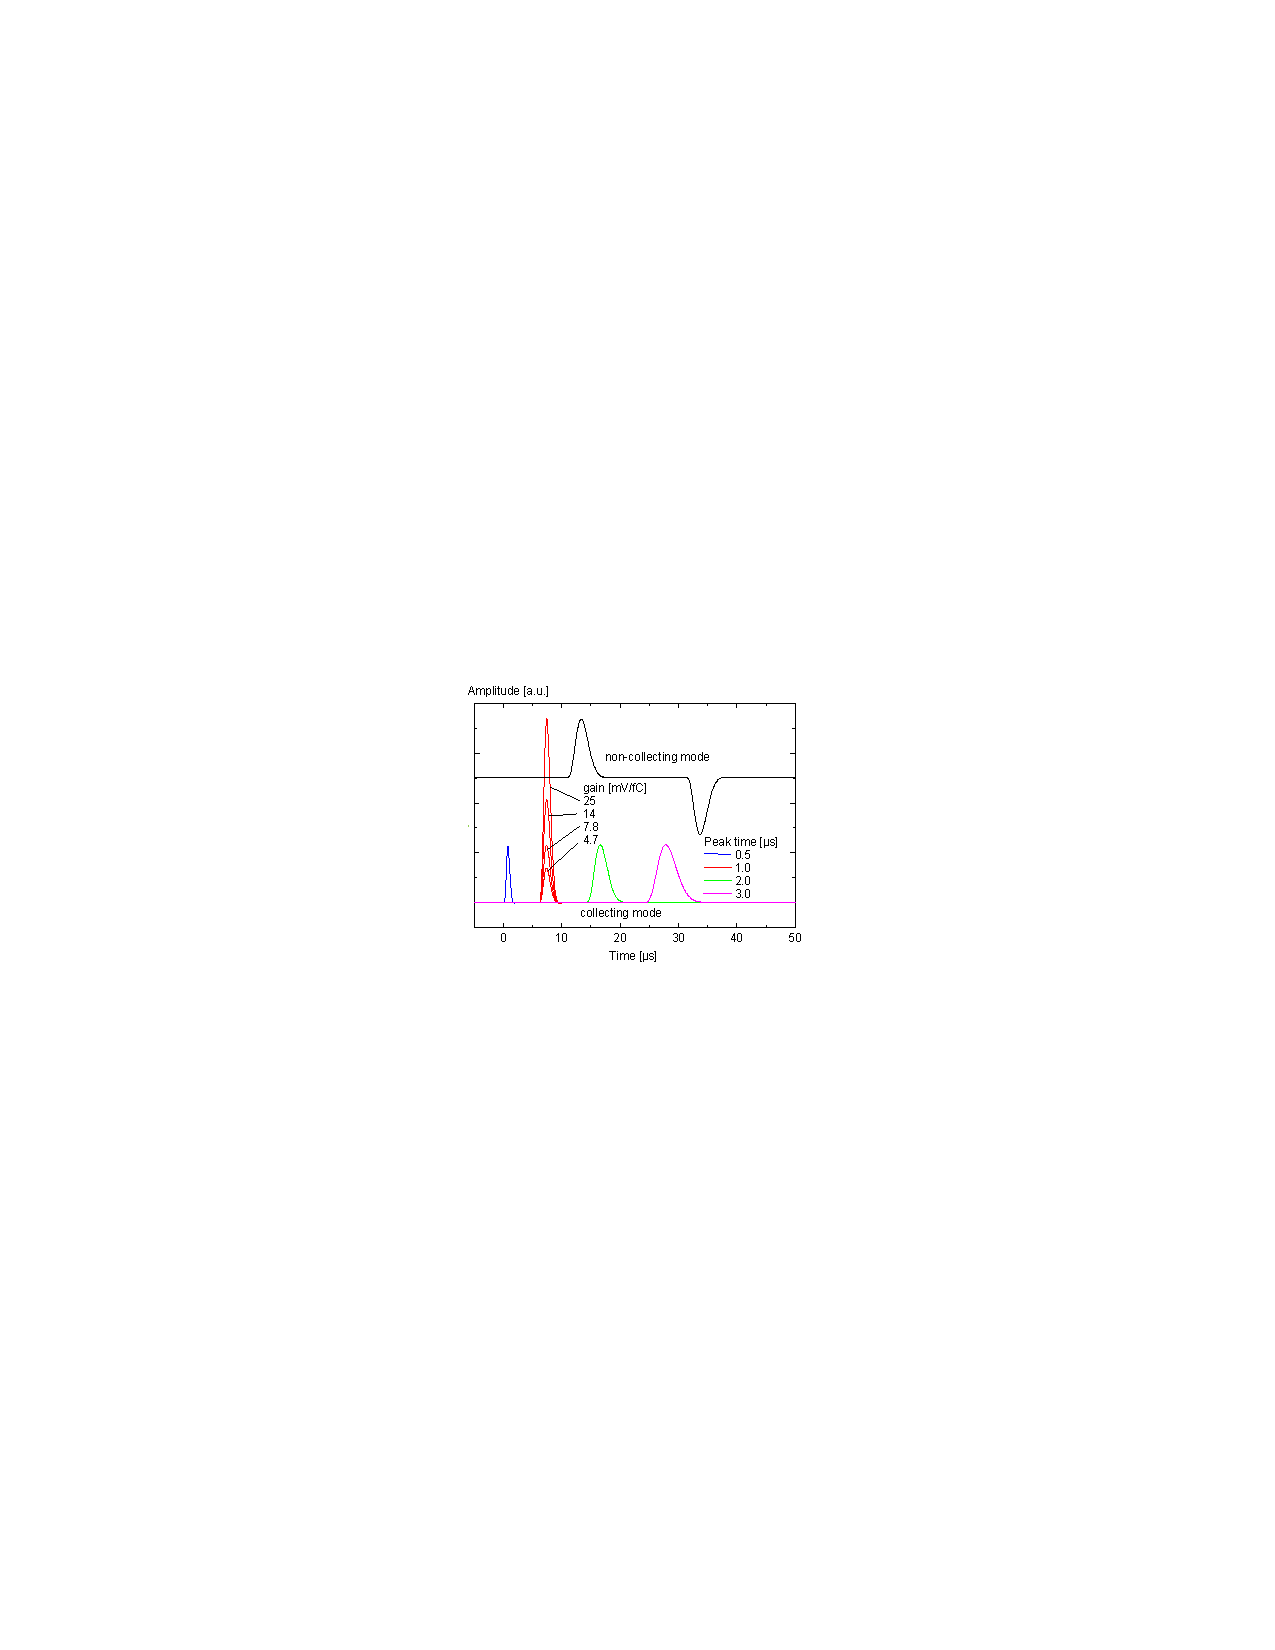
\includegraphics[width=0.47\linewidth]{tpcelec-shaper_out.pdf}
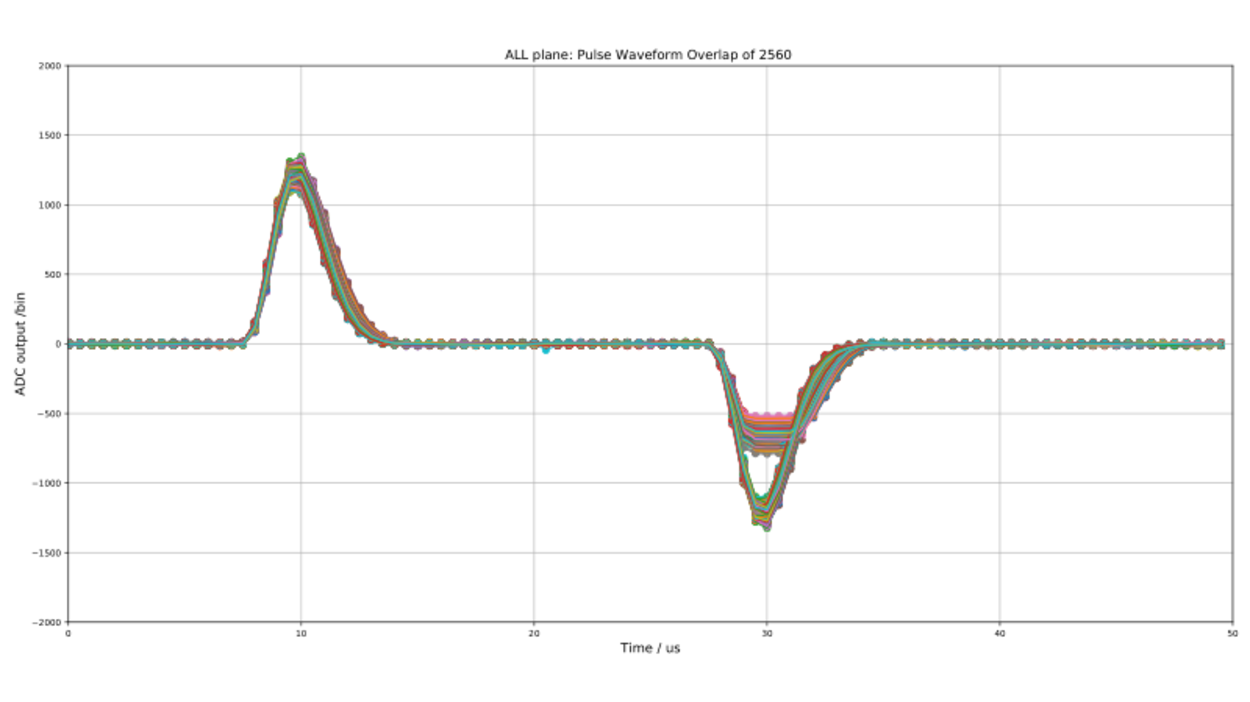
\includegraphics[width=0.5\linewidth]{tpcelec-pdune-wf.pdf}
\end{dunefigure}

Each FE LArASIC channel is equipped with an injection capacitor which can be used
for test and calibration and can be enabled or disabled through a
dedicated register. The injection capacitance has been measured to 0.5$\%$ using 
a calibrated external capacitor. The measurements show
that the calibration capacitance is extremely stable, changing from
184~fF at room temperature to 183~fF at 77~K. This result and the measured
stability of the peaking time demonstrate the high stability of the
passive components as a function of temperature. Channel-to-channel and chip-to-chip
variation in the calibration capacitor are typically less than 1\%. 

Prototype LArASIC have been evaluated and characterized at room temperature (300~K) and LN$_2$
(77~K) temperature.
During testing the circuits have been cycled multiple times
between the two temperatures and operated without any change in performance.
Figure~\ref{fig:fe-output} (right) shows the measured injection pulse response overlayed with the baseline subtracted for one full APA 
(2,560) electronics channels from ProtoDUNE-SP FEMB attached to a ProtoDUNE-SP APA in a 
shielded environment at approximately 180 degrees Kelvin. This contains 1,600 induction (high-baseline)
and 960 collection (low-baseline) channels, the latter of which saturate the negative pulse at the low 
end of the FE output. The spread in saturization values between -500 and -750 ADC bins is due to the
variation in relative position of the FE baseline to the low end of the FE output 
in the ProtoDUNE-SP version of the LArASIC.
%These results are in close agreement with simulations and indicate
%that both the analog and the digital circuits and interface operate as
%expected in a cryogenic environment.



